% !TeX spellcheck = da_DK
\chapter{Kroppens balance}\label{app-Balance}
Apopleksi patienter oplever ofte problemer med balancen, da den ofte er nedsat eller slet ikke funktionsdygtig af forskellige årsager. \cite{Karnath2003} Proprioceptorer og sansereceptorer hjælper kroppen med balancen. Proprioceptorerne kontrollerer muskler, sener og leds position, hvorimod sansereceptorer er en bestemt slags celler, som er placeret i ørerne og øjnene. \cite{Martini2012} Disse celler sender balanceinformationer til det centrale nervesystem og hjernen. Sansereceptorerne opfanger indtryk fra sanserne, som omsættes til bestemte signaler, der sendes til områder i cerebral cortex, cerebellum og til centre i hele hjernestammen. Her bearbejdes informationen, hvorefter der konkluderes den korrekte fysiske position af kroppen og dens lemmer. Når hjernen har bearbejdet indtrykkene, udsender den nerveimpulser til skeletmuskulaturen om at foretage jævne og koordinerede bevægelser, hvorved kropsbalancen opretholdes.\cite{Martini2012} Der ses et flowdiagram af samarbejdet imellem proprioceptorer og sansereceptorer i øjne og øret på \figref{flowbalance}. \\
Øjne opfanger lys og er med til orienteringen af kroppen og dens lemmer. Hårceller i øret register derimod f.eks. hoveds bevægelser vha. tyngdekraften. Selvom et balanceorgan er ude af funktion, er kroppen stadig i stand til at opretholde balancen ved hjælp fra andre balanceorganer. Det er til gengæld vanskeligt for kroppen at opretholde balancen, hvis de behandlende centre i hjernen bliver skadet, som det kan ske ved apopleksi patienter. \cite{Martini2012} \\
\fxnote{MADS - MANGLER KILDE TIL FLOWDIAGRAM}
\begin{figure}[H]
	\centering
	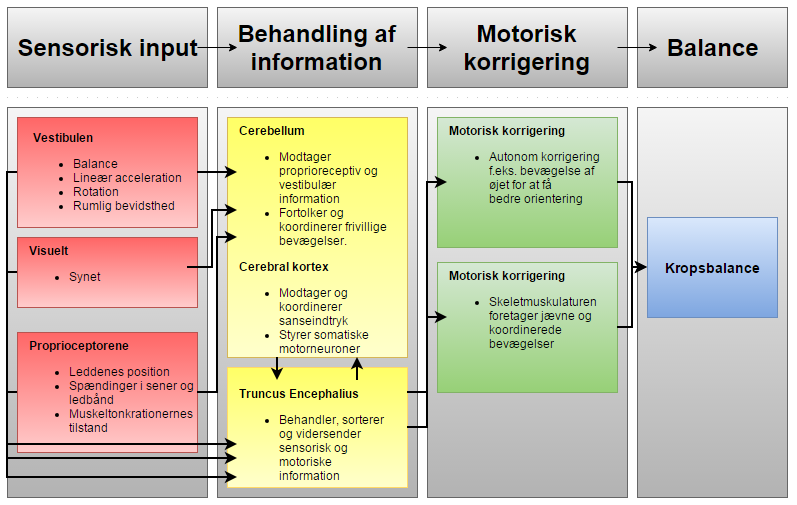
\includegraphics[scale=0.4]{figures/bProblemanalyse/Balance-Flowdiagram.png}
	\caption{På dette flowdiagram ses, hvordan synet, hørelsen og propioreceptorer samarbejder for at opretholde kropsbalancen. }
	\label{flowbalance}
\end{figure}

\section{Ørets bidrag til balance}
Øret består overordnet af tre dele; det ydre øre, mellemøret og det indre øre, som kan ses på \figref{Oeret}. Det indre øre er med til at kontrollere balancen vha. hårcellerne, som sættes i bevægelse. Det ydre øre modtager trykbølger, som sætter trommehinden i svingninger. Disse transporteres af mellemørets knogler, der forstærker svingningerne. Væsken i mellemøret modtager svingningerne fra knoglerne, hvilket sætter væsken i bevægelse. Denne bevægelse trækker i hårcellerne, og der skabes derved et aktionspotentiale. I det indre øre findes et netværk af sammenhængende væskeholdige kanaler, som er indkapslet i knoglen. Det er i disse kanaler receptorerne sidder. Det indre øre kan opdeles i tre underdele; vestibulen, øresneglen og buegangen. De centrale dele, der har med balancen at gøre er vestibulen og buegangen, hvorimod øresneglen kun bidrager til hørelsen.\cite{Martini2012}  \\
Vestibulen består af to membransække; sacculen og utriclen, der opfanger sanseindtryk vedrørende tyngdekraft og lineær acceleration. Buegangens sansereceptorer opfanger stimuli omkring hovedets bevægelse, og hvor hurtigt bevægelsen foregår. Sansereceptorerne er placeret i buegangens tre væskefyldte knoglekanaler ved ampulla, der er forbundet til utriclen. Hårcellerne er kun aktive, når kroppen er i bevægelse ved at videregive information vedrørende hovedets bevægelse ift. tyngdekraften. Når hovedet er i bevægelse, sættes væskens i kanalerne også i bevægelse således, at væskebevægelser i den ene retning stimulerer hårcellerne, mens bevægelser i den modsatte retning forhindrer dem. For at få mest mulig information angående hovedets position, stimuleres de tre buegange af forskellige hovedbevægelser. Bevægelsesinformationerne sendes via vestibulocochlearnerven, der sender både information vedrørende balancen og hørelsen til hjernen i områder i pons og medulla oblongata. \cite{Martini2012}    

\begin{figure}[H]
	\centering
	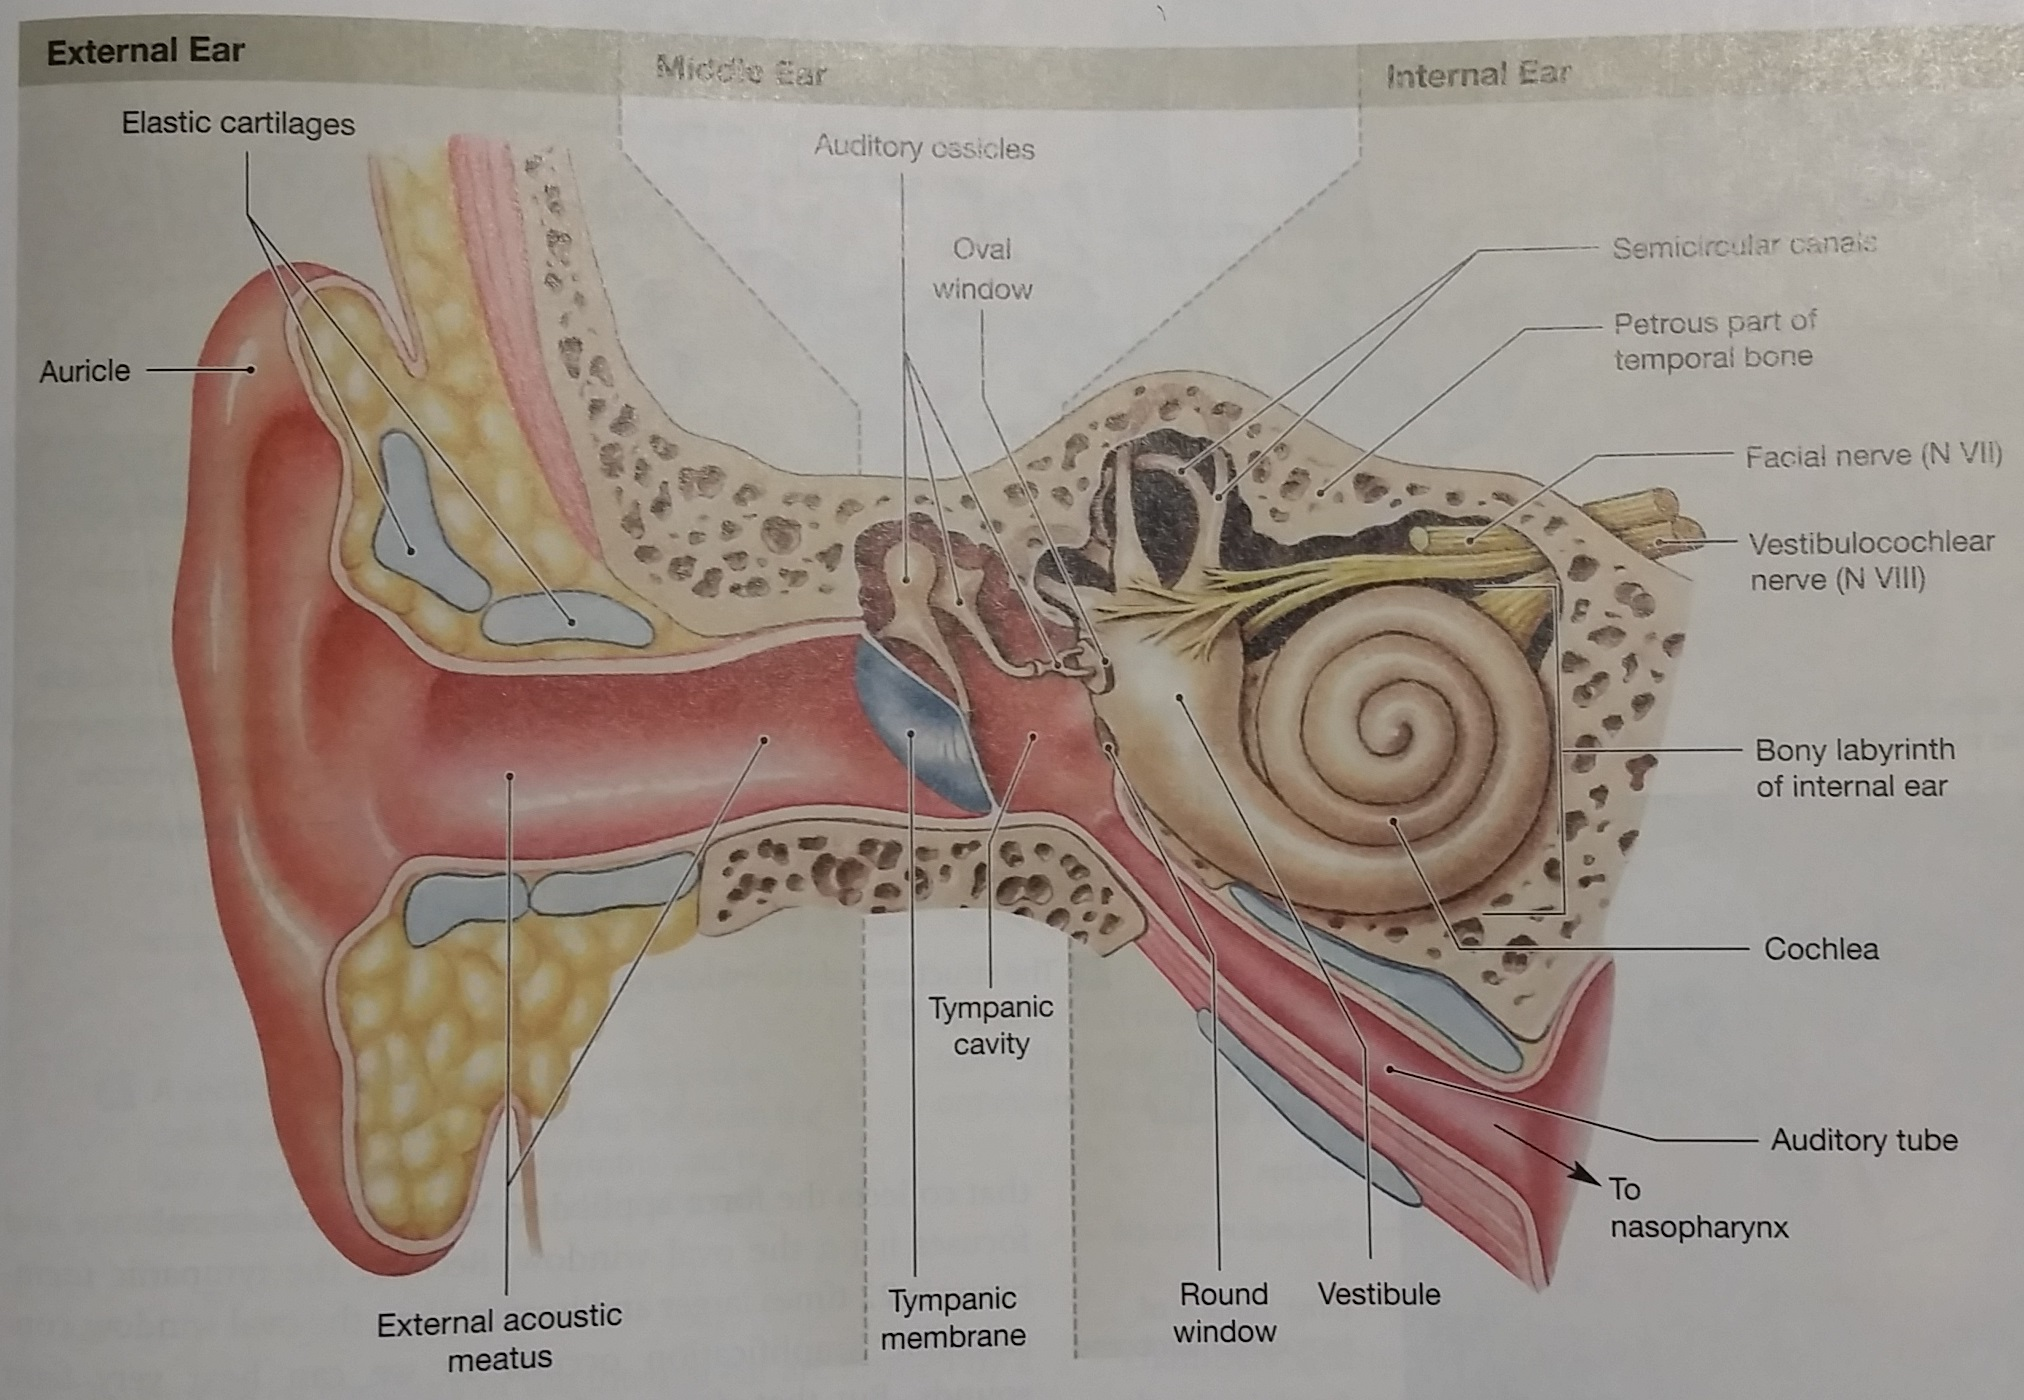
\includegraphics[scale=0.75]{figures/bProblemanalyse/Oerets-anatomi.jpg}
	\caption{På billedet ses en anatomisk beskrivelse af øret. \cite{Martini2012}}
	\label{Oeret}
\end{figure}

\section{Øjets bidrag til balance}
Synet er en central faktor for, hvordan hjernen holdes informeret omkring kroppens balance og generel orientering. Dette gøres ved at give et indtryk af, hvordan kroppen og dens lemmer er placeret ift. omgivelserne\fxnote{Mads kilde - HUSK HUSK HUSK}. Øjet har tre hinder omkring sig; fibrøs hinde, uvea og retina, som kan ses på \figref{Oejet}. Den fibrøse hinde\fxnote{hornhinden} er den yderste, som beskytter og støtter øjet. Den midterste hinde, kaldet uvea, indeholder blod og lymfekar samt regulerer mængden af lys, der kommer ind i øjet. Retina\fxnote{nethinden} er den inderste hinde, som er placeret bagerst i øjet. Den består af en pigmentdel og en indre neuraldel. Den neurale del indeholder fotoreceptorer, kaldet stave og tappe. Stave er følsomme overfor skarp lys og gør, at vi kan se i tusmørke. Tappe er følsomme overfor farvers bølgelængde, hvilket giver os farvesyn. Pigmentdelen absorberer lys, der passerer gennem den neurale del og gør, at lyset ikke har mulighed for at reflektere tilbage. Foto- og lysreceptorerne konverterer lyset fra omgivelserne til elektrisk nervesignal, der giver information omkring det objekt, der betragtes, herunder dets størrelse, form og bevægelser. Informationerne processeres således, at horiensontale celler lokaliserer områdets størrelse. Hvis der er kommet nok signal ind, der kræver en reaktion, sendes informationen først til bipolære celler herefter via synsnerven til den visuelle cortex, hvor informationen bearbejdes. \cite{Martini2012}     

\begin{figure}[H]
	\centering
	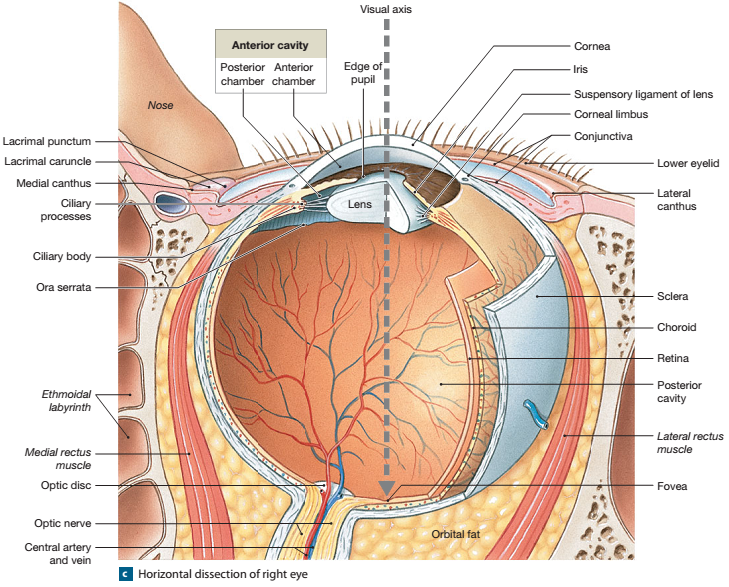
\includegraphics[scale=0.75]{figures/bProblemanalyse/Oejets-anatomi.png}
	\caption{På billedet ses en anatomisk beskrivelse af øjet. \cite{Martini2012}}
	\label{Oejet}
\end{figure}

\section{Proprioceptorerne og skeletmuskulaturens indvirkning på balancen}
Proprioceptorer monitorer leddenes position, muskelkontraktioners tilstand, samt spændinger i ledbånd og sener og de er placeret i skeletmuskulaturen. Informationerne sendes via nervesignaler til rygmarven og herfra igennem CNS til cerebellum. Proprioceptorer inddeles i tre overordnet grupper; muskelspindlere, golgi-sene organer og receptorer i ledkapsler.\cite{Martini2012}    \\
Muskelspindlere styrer og kontrollerer ændringer af muskellængder og kan udløse en strækrefleks. Den sensoriske nerve er forbundet centralt på muskelspindleren, hvor den kontinuert sender sensoriske impulser til CNS. Hvis den sensoriske nerve modtager stimuli, i form af stræk, vil den motoriske nerve på muskelspindleren blive stimuleret. Stimulation af den motoriske nerve vil forkorte musklens længde. Nogle strækreflekser er holdningsreflekser, som hjælper os med at holde balancen. I en stående position kræves der samarbejde mellem mange forskellige muskelgrupper for at forblive stående. Dette ses f.eks. hvis kroppen lænes forover, vil strækreflekserne i læggene blive aktiveret og kontraherer. Derved vil kroppen læne sig bagud og igen stå i en opret position. Hvis der sker en overkompensation fra lægmusklerne og kroppen læner sig for meget bagud, vil strækreflekser i skinnebenet og lårene aktiveres. Derved vil kroppen læne sig forover igen. Kroppen foretager mange af disse ubevidste korrektioner. \cite{Martini2012}   \\ %(Se Martini 9th side 438 under "monosynaptic reflexes")
Golgi-sene organer sidder i en kløft\fxnote{junction} mellem skeletmusklen og tilhørende sene. Dendritterne fra golgi-sene organet kopler sig på den tætteste sene og stimuleres af spændingen i denne, hvorved den eksterne spænding i en muskelkontraktion bliver målt. \cite{Martini2012}    \\
Ledkapsler er fyldt med frie nerveender, som kaldes receptorer. Disse receptorer detekterer tryk, spænding og bevægelse i leddet. \cite{Martini2012}    \\
Det er kun en lille del, af den information proprioceptererne sender, der opfanges af bevidstheden, eftersom størstedelen foregår på et underbevidst niveau.\cite{Martini2012} \\


%Golgi seneorganer (Se Martini 9th side 501 under 15-3 propriocetor) %Receptorer i ledkapsler (Se Martini 9th side 501 under 15-3 propriocetor)

%\subsection{Apopleksi og balance}
%Balancen er styrer flere steder i kroppen og er med til at beskytte kroppen mod f.eks. faldulykker, ved at sikre at kroppen og den lemmer bevæger sig i kontrollerede og jævne bevægelser. Kroppen opretholder balancen ved at bruge ørerne, øjne og proprioceptorer i skeletmuskulaturen. Proprioceptorerne kontrollerer muskler, sener og leds position. Øjne opfanger lys og er med til orienteringen af kroppen og dens lemmer og hårceller i øret register hoveds bevægelser ved hjælp af tyngdekraften. Selvom et balanceorgan er ude af funktion er kroppen stadig i stand til at opretholde balancen ved hjælp fra andre balanceorganer. Det er til gengæld svære for kroppen at opretholde balancen hvis centrene i hjerne, som behandler den information, som kommer fra balanceorganerne, bliver skadet, som det kan ske ved apopleksi patienter. \cite{Martini2012}
% [1] – Martini, Frederic H and others. Fundamentals of Anatomy & Physiology (Kapitel:13, 14, 15, 17 ). 2012. Pearson. 
% [2] - Karnath2003